\documentclass{article} % Change to a standard article class
\usepackage{amsmath} % for math environments and commands
\usepackage{cite}
\usepackage{amssymb}
\usepackage{amsfonts}
\usepackage{graphicx}
\usepackage{textcomp}
\usepackage{xcolor}

\begin{document}

\title{K Nearest Neighbors\\
\thanks{Insert applicable funding agency here. If none, delete this.}
}

\author{Arthur Felipe Reis Souza \\
Electrical Engineering Department, \\
Federal University of Minas Gerais, \\
Belo Horizonte, Brazil \\
arthurfreisouza@gmail.com \\
\and
Antônio de Pádua Braga and Frederico Gualberto Ferreira Coelho \\
Electrical Engineering Department, \\
Federal University of Minas Gerais, \\
Belo Horizonte, Brazil \\
apbraga@cpdee.ufmg.br, fredgfc@ufmg.br
}

\maketitle

\begin{abstract}

    Esse relatório tem por objetivo demonstrar o algoritmo de Machine Learning K-Nearest Neighbors (KNN), suas vantagens, desvantagens e aplicações.

\end{abstract}

\section{Introdução}

O algoritmo K-Nearest Neighbors (KNN) é amplamente utilizado em Machine Learning tanto para tarefas de classificação quanto de regressão. No contexto de classificação, ele se baseia em um número K de vizinhos mais próximos e nos rótulos desses vizinhos para tomar a decisão. Ao classificar um novo ponto P, primeiro calcula-se a distância entre esse ponto e todos os outros do conjunto de dados. Em seguida, considera-se os rótulos correspondentes aos K vizinhos mais próximos, definidos pelas menores distâncias, para determinar o rótulo do novo ponto. No caso de classificação, o ponto classificado será decidido com base na moda dos valores, enquanto no caso de regressão, o algoritmo pegará a média dos K rótulos mais próximos.

\vspace{1cm}

\begin{figure}[h] % 'h' posiciona a figura aproximadamente no local do código
    \centering % centraliza a figura
    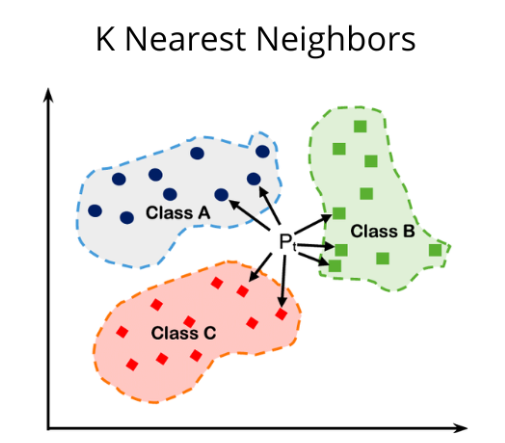
\includegraphics[width=0.5\linewidth]{KNN_pic.png} % insira o caminho da sua imagem e ajuste a largura
    \caption{Algoritmo KNN.} % insira a legenda desejada
    \label{fig:exemplo} % rótulo para referenciar a figura no texto
\end{figure}

\vspace{1cm}

O algoritmo K-Nearest Neighbors (KNN) é um método baseado em distância, o que o torna sensível tanto à normalização dos dados quanto à escolha da métrica de distância utilizada. Existem diversas métricas que podem ser aplicadas neste algoritmo; neste relatório, optamos pela distância euclidiana, que é expressa pela equação $\sqrt{\sum_{i=1}^{n} (x_i - y_i)^2}$.

\vspace{1cm}

Um fator crucial que influencia o desempenho do classificador é a escolha do número de vizinhos mais próximos, representado pelo valor de K. Valores baixos de K tendem a resultar em um desempenho insatisfatório devido ao fenômeno de overfitting, já que o algoritmo considera apenas o rótulo mais próximo. Por outro lado, valores altos de K também podem comprometer o desempenho do classificador, pois o algoritmo leva em conta todo o conjunto de dados, diluindo a relevância dos rótulos mais próximos e sendo também influenciado pelo viés dos dados, ou seja, se uma das classes tem mais amostras ela irá influenciar mais no desempenho do modelo. Portanto, é fundamental determinar um valor ideal de K. Isso pode ser alcançado por meio do algoritmo Grid Search, que explora uma grade de diferentes valores de K e avalia o desempenho do classificador utilizando o método de Cross-Validation.

\section{Geração dos dados}

Os dados foram gerados com base em distribuições normais, caracterizadas pela média e pelo desvio padrão. Um alto desvio padrão pode resultar na sobreposição das amostras de ambas as classes, dificultando a classificação pelo algoritmo. Em contraste, um baixo desvio padrão tende a gerar classes mais linearmente separáveis, o que favorece o desempenho do classificador. Abaixo, apresentamos imagens que ilustram as duas situações: na primeira, não há superposição entre as classes, enquanto na segunda, um alto desvio padrão resulta em sobreposição.

\vspace{1cm}

\begin{figure}[h] % 'h' posiciona a figura aproximadamente no local do código
    \centering % centraliza a figura
    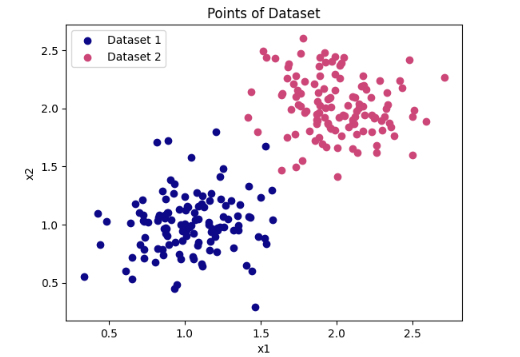
\includegraphics[width=0.5\linewidth]{KNN_sigma_0.25.png} % insira o caminho da sua imagem e ajuste a largura
    \caption{Dados com baixo desvio padrão $\sigma$ = 0,25.} % insira a legenda desejada
    \label{fig:exemplo} % rótulo para referenciar a figura no texto
\end{figure}

\vspace{1cm}

É notório acima que as classes são linearmente separáveis.

\vspace{1cm}

\begin{figure}[h] % 'h' posiciona a figura aproximadamente no local do código
    \centering % centraliza a figura
    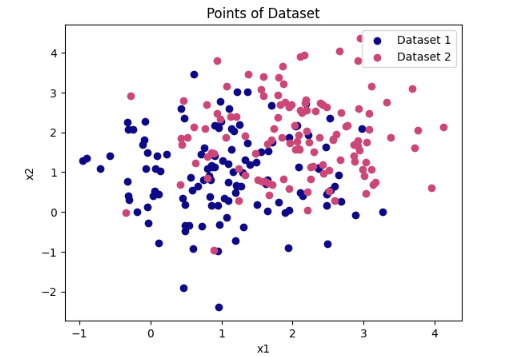
\includegraphics[width=0.5\linewidth]{KNN_sigma_1.png} % insira o caminho da sua imagem e ajuste a largura
    \caption{Dados com alto desvio padrão $\sigma$ = 1.} % insira a legenda desejada
    \label{fig:exemplo} % rótulo para referenciar a figura no texto
\end{figure}

\vspace{1cm}

Acima é possível observar que com o desvio padrão $\sigma$  mais alto há a superposição das duas classes, influenciando no desempenho do classificador.

\section{Função KNN}

Esta seção tem como objetivo descrever a função do KNN tradicional, que é considerado mais simples, pois não possui parâmetros que previnem o underfitting e o overfitting. A seguir, apresentamos a implementação em Python da função do KNN, acompanhada de uma descrição detalhada, passo a passo, de seu funcionamento.

\vspace{1cm}

\begin{figure}[h] % 'h' posiciona a figura aproximadamente no local do código
    \centering % centraliza a figura
    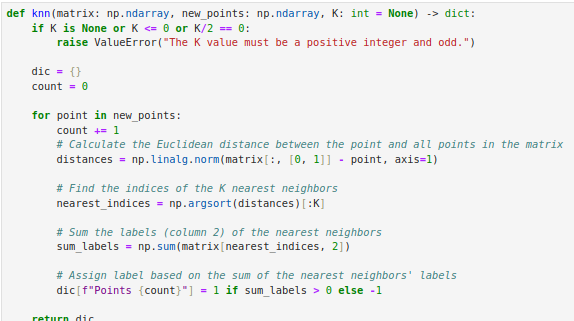
\includegraphics[width=0.75\linewidth]{KNN_function.png} % insira o caminho da sua imagem e ajuste a largura
    \caption{Implementação da função do KNN.} % insira a legenda desejada
    \label{fig:exemplo} % rótulo para referenciar a figura no texto
\end{figure}

\vspace{1cm}

\begin{enumerate}
    \item \textbf{Calcular a distância entre o ponto de teste e todos os pontos do conjunto de dados.} Para isso, pode-se utilizar a distância Euclidiana ou outra métrica de distância.
    
    \item \textbf{Selecionar os K vizinhos mais próximos.} A partir das distâncias calculadas, escolha os K pontos que têm as menores distâncias em relação ao ponto de teste.
    
    \item \textbf{Contar os rótulos dos K vizinhos selecionados.} Após selecionar os vizinhos, verifique os rótulos correspondentes a esses pontos.
    
    \item \textbf{Determinar o rótulo do ponto de teste.} O rótulo do ponto de teste será o que aparecer com mais frequência entre os K vizinhos. Caso haja um empate, pode-se usar uma estratégia para decidir, mas no geral há uma restrição nos valores de K, sendo o mesmo um valor ímpar.
    
    \item \textbf{Retornar o rótulo classificado.} Por fim, a função deve retornar o rótulo determinado para o ponto de teste.
\end{enumerate}

\section{Geração de novos dados}

Novos dados foram gerados para realizar a inferência do modelo, abaixo estão os novos dados gerados considerando $\sigma$ = 0.25 e $\sigma$ = 1.

\vspace{1cm}

\begin{figure}[h] % 'h' posiciona a figura aproximadamente no local do código
    \centering % centraliza a figura
    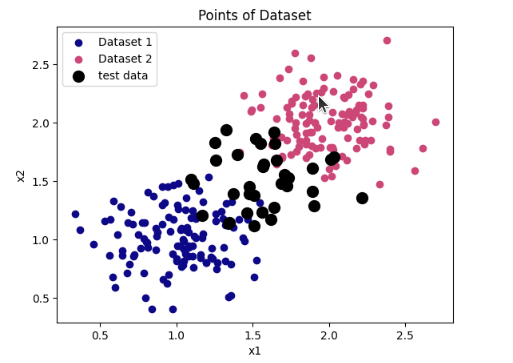
\includegraphics[width=0.5\linewidth]{KNN_test_sigma_0.25.png} % insira o caminho da sua imagem e ajuste a largura
    \caption{Gráfico com novos dados para a classificação considerando $\sigma$ = 0.25.} % insira a legenda desejada
    \label{fig:exemplo} % rótulo para referenciar a figura no texto
\end{figure}

\vspace{1cm}

\begin{figure}[h] % 'h' posiciona a figura aproximadamente no local do código
    \centering % centraliza a figura
    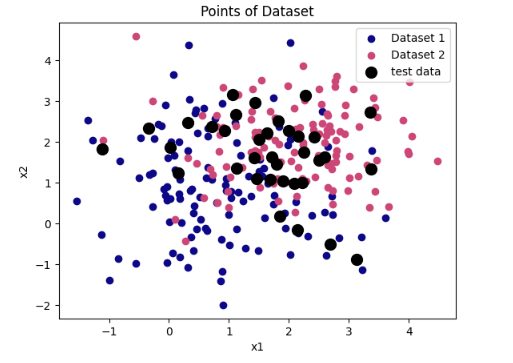
\includegraphics[width=0.5\linewidth]{KNN_test_sigma_1.png} % insira o caminho da sua imagem e ajuste a largura
    \caption{Gráfico com novos dados para a classificação considerando $\sigma$ = 1.} % insira a legenda desejada
    \label{fig:exemplo} % rótulo para referenciar a figura no texto
\end{figure}

\vspace{1cm}

A principal ideia é utiliar esses novos dados de testes para realizar a inferência do classificador e avaliar como o mesmo os classificará, plotando a classificação resultante e também a superfície de separação ao variar os parâmetros K.

\section{Resultados}

Os resultados abaixo mostram os resultados do classificador sobre os dados de teste, utilizando k = 3.

\vspace{1cm}

\begin{figure}[h] % 'h' posiciona a figura aproximadamente no local do código
    \centering % centraliza a figura
    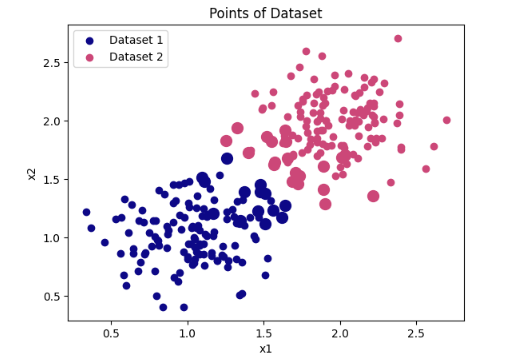
\includegraphics[width=0.5\linewidth]{result_KNN_test_sigma_0.25.png} % insira o caminho da sua imagem e ajuste a largura
    \caption{Resultado da classificação com $\sigma$ = 0.25 e K = 3.} % insira a legenda desejada
    \label{fig:exemplo} % rótulo para referenciar a figura no texto
\end{figure}

\begin{figure}[h] % 'h' posiciona a figura aproximadamente no local do código
    \centering % centraliza a figura
    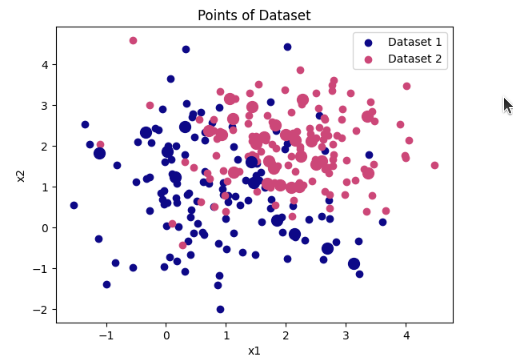
\includegraphics[width=0.5\linewidth]{result_KNN_test_sigma_1.png} % insira o caminho da sua imagem e ajuste a largura
    \caption{Resultado da classificação com $\sigma$ = 1 e K = 3.} % insira a legenda desejada
    \label{fig:exemplo} % rótulo para referenciar a figura no texto
\end{figure}

A variação do valor de K, tanto para valores baixos quanto para altos, não resultou em diferenças significativas na classificação dos dados de teste. No entanto, essa variação permite analisar como a superfície de separação se altera, possibilitando a identificação de fenômenos como overfitting e underfitting. A seguir, apresentamos gráficos que utilizam K = 1 e $\sigma$ = 0.25, evidenciando um potencial overfitting do modelo. Embora o overfitting não seja claramente perceptível devido à linearidade dos dados, o modelo ainda consegue discriminar bem as classes, mesmo com valores baixos de K. Em contraste, ao adotar um valor maior de K, como K = 3, a superfície de separação torna-se mais estável, contribuindo para a mitigação do overfitting.

\begin{figure}[h] % 'h' posiciona a figura aproximadamente no local do código
    \centering % centraliza a figura
    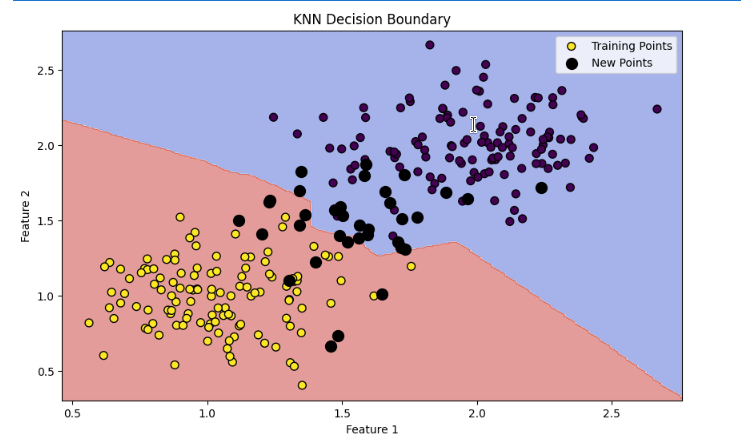
\includegraphics[width=0.5\linewidth]{separation_surface_K1_sigma_025.png} % insira o caminho da sua imagem e ajuste a largura
    \caption{Superfície de separação com $\sigma$ = 0.25 e K = 1.} % insira a legenda desejada
    \label{fig:exemplo} % rótulo para referenciar a figura no texto
\end{figure}

\begin{figure}[h] % 'h' posiciona a figura aproximadamente no local do código
    \centering % centraliza a figura
    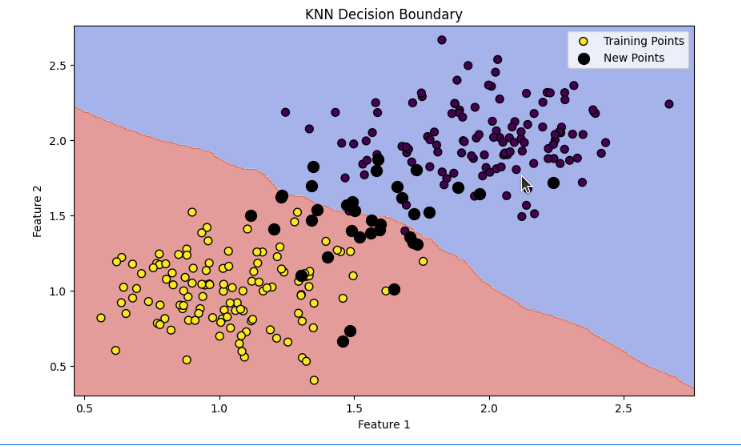
\includegraphics[width=0.5\linewidth]{separation_surface_K7_sigma_025.png} % insira o caminho da sua imagem e ajuste a largura
    \caption{Superfície de separação com $\sigma$ = 0.25 e K = 3.} % insira a legenda desejada
    \label{fig:exemplo} % rótulo para referenciar a figura no texto
\end{figure}

\newpage

No fito de observar como o overfitting do modelo, aumenta-se o desvio padrão $\sigma$ para 1, onde haverá uma maior superposição entre os dados, tornando o mesmo mais visível. Abaixo estarão as superfícies de separação para valores de K = 1, K = 3, K = 7 e K = 51.

\begin{figure}[h] % 'h' posiciona a figura aproximadamente no local do código
    \centering % centraliza a figura
    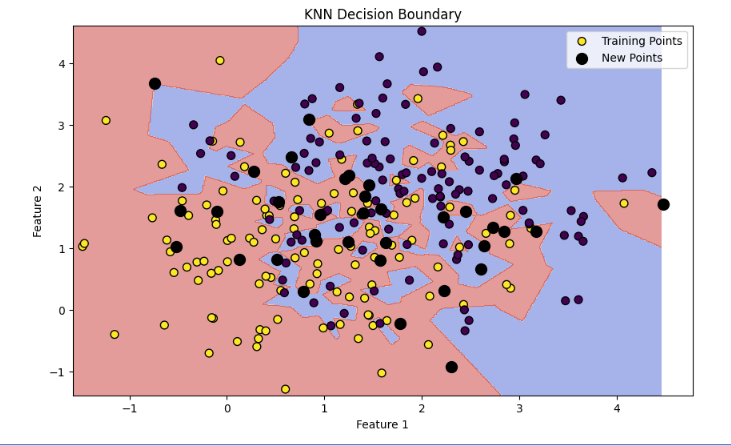
\includegraphics[width=0.5\linewidth]{separation_surface_sigma1_k1.png} % insira o caminho da sua imagem e ajuste a largura
    \caption{Superfície de separação com $\sigma$ = 1 e K = 1.} % insira a legenda desejada
    \label{fig:exemplo} % rótulo para referenciar a figura no texto
\end{figure}

\begin{figure}[h] % 'h' posiciona a figura aproximadamente no local do código
    \centering % centraliza a figura
    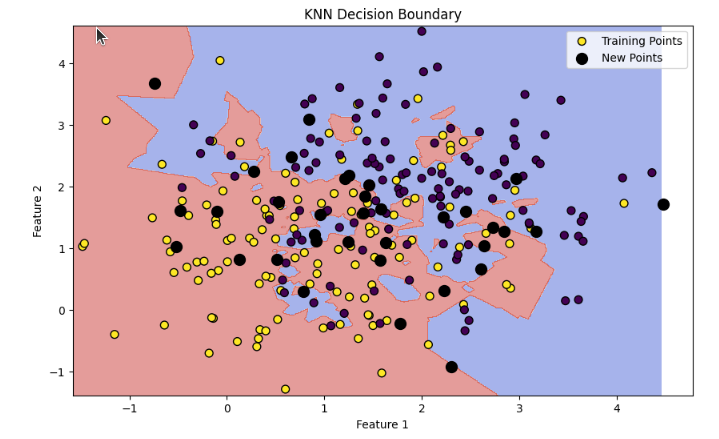
\includegraphics[width=0.5\linewidth]{separation_surface_sigma1_k3.png} % insira o caminho da sua imagem e ajuste a largura
    \caption{Superfície de separação com $\sigma$ = 1 e K = 3.} % insira a legenda desejada
    \label{fig:exemplo} % rótulo para referenciar a figura no texto
\end{figure}

\begin{figure}[h] % 'h' posiciona a figura aproximadamente no local do código
    \centering % centraliza a figura
    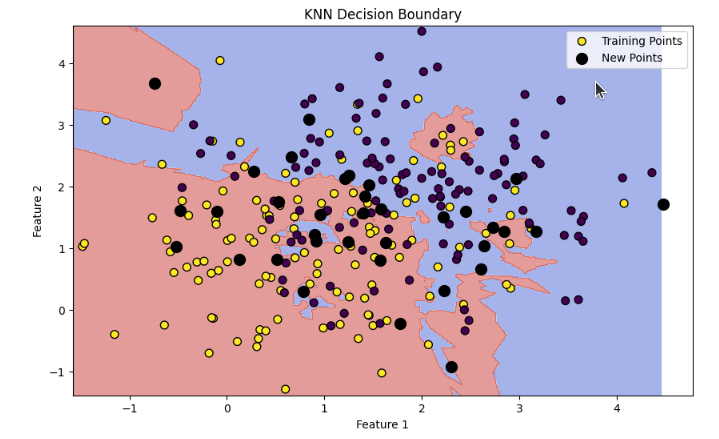
\includegraphics[width=0.5\linewidth]{separation_surface_sigma1_k7.png} % insira o caminho da sua imagem e ajuste a largura
    \caption{Superfície de separação com $\sigma$ = 1 e K = 7.} % insira a legenda desejada
    \label{fig:exemplo} % rótulo para referenciar a figura no texto
\end{figure}

\begin{figure}[h] % 'h' posiciona a figura aproximadamente no local do código
    \centering % centraliza a figura
    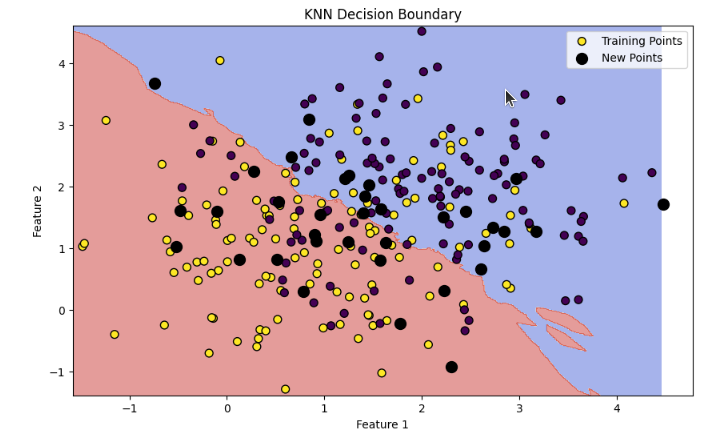
\includegraphics[width=0.5\linewidth]{separation_surface_sigma1_k51.png} % insira o caminho da sua imagem e ajuste a largura
    \caption{Superfície de separação com $\sigma$ = 1 e K = 51.} % insira a legenda desejada
    \label{fig:exemplo} % rótulo para referenciar a figura no texto
\end{figure}

\newpage

Pode se notar, ao analisar os dados acima é que, aumentando o valor de K reduz o efeito do overfitting nesse conjunto de dados os quais estão superpostos com $\sigma$ = 1. O efeito do overfitting agora é claramente visto com K = 1, K = 3 e também K = 7, enquanto o efeito do mesmo é reduzido consideravelmente ao se utilizar um alto de valor de K, sendo ele K = 51. Vale ressaltar também que a escolha do valor de K depende da base de dados e também da superposição do mesmo, para os dados utilizados, os quais estão superpostos, o valor de K que irá mitigar o overfitting tem um valor alto, mas para base de dados que são linearmente separáveis, o valor de K tenderá a ser menor.

\newpage

\section{Conclusão}

Portanto, ao finalizar o exercíco é possível observar e estudar o algoritmo K Nearest Neighbors, o qual é totalmente sensível ao valor de K e também a métrica de distância utilizada. O desempenho do modelo depende totalmente de como os dados estão superpostos, e o valor de K dependerá também dessa informação. Como pode se observar na figura acima, baixos valores de K em um conjunto de dados superposto acarreta em overfitting, enquanto para um conjunto não superposto não acarreta, pois os dados são facilmente linearmente separáveis. Outro fator que influencia bastante o desempenho do modelo é se os dados estão ou não normalizados, considerando-se que é  um modelo baseado em distância.

\end{document}
